\documentclass[tikz,border=6pt]{standalone}
\usepackage[T1]{fontenc}
\usepackage[utf8]{inputenc}
\usepackage{lmodern}
\usetikzlibrary{arrows.meta,fit,backgrounds,calc}
\definecolor{blue}{RGB}{40,96,128}
\definecolor{green}{RGB}{63,117,93}
\begin{document}
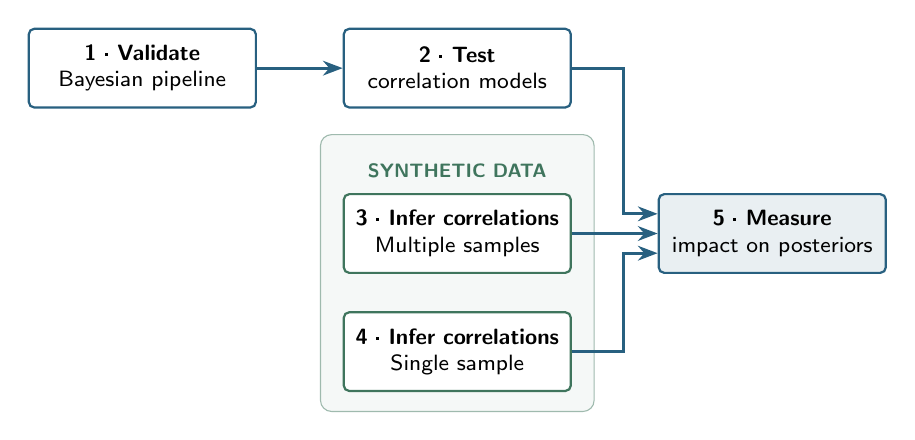
\begin{tikzpicture}[
 box/.style={draw=blue,fill=white,rounded corners=2pt,line width=.8pt,
 text width=2.65cm,minimum height=1cm,align=center,font=\sffamily\footnotesize},
 arrow/.style={-{Stealth[length=2.5mm]},line width=1pt,draw=blue}
]
\node[box] (p1) at (0,2.1) {\textbf{1 · Validate}\\Bayesian pipeline};
\node[box] (p2) at (4,2.1) {\textbf{2 · Test}\\correlation models};
\node[box,draw=green] (p3) at (4,0) {\textbf{3 · Infer correlations}\\Multiple samples};
\node[box,draw=green] (p4) at (4,-1.5) {\textbf{4 · Infer correlations}\\Single sample};
\node[box,fill=blue!10] (p5) at (8,0) {\textbf{5 · Measure}\\impact on posteriors};
\node[font=\sffamily\bfseries\scriptsize,text=green] (data) at (4,.8)
 {SYNTHETIC DATA};
\begin{scope}[on background layer]
 \node[fit=(p3)(p4)(data),inner xsep=8pt,inner ysep=7pt,
 draw=green!50,fill=green!5,rounded corners=4pt] (parallel) {};
\end{scope}
\draw[arrow] (p1.east) -- (p2.west);
\draw[arrow] (p2.east) -- ++(.65,0) |- ($(p5.west)+(0,.25)$);
\draw[arrow] (p3.east) -- (p5.west);
\draw[arrow] (p4.east) -- ++(.65,0) |- ($(p5.west)+(0,-.25)$);
\end{tikzpicture}
\end{document}
